\chapter{Cross Section Measurement}

The cross section measurement procedure and results are explained in this section.
After applying selection criteria and kinematic reconstruction, one can count the events to determine
the rate of $t\bar{t}$ production process.

The cross sections were measured double differentially in bins of the kinematic variables of the event.
A binning choice is explained in the first section.
The two dimensional unfolding was applied to correct for the detector effect and fluctuations, which is described
in the second section of this chapter.
The double differential cross sections and their definitions are shown in the last section of the chapter.
% \section{Selection of Binning}\label{sec:binning}

\section{Background Subtraction}
This study is performed as counting the events which fulfill certain criteria (e.g. given in chapter \ref{chapt:event_selection} and 
chapter \ref{chapt:kinReco}). Not all of these events are originating from the $t\bar{t}$ system decay in dileptonic
channel. The final state, which can be misidentified as $t\bar{t}$, may arise from a different process, called \textit{background}
for the specific measurement. In this analysis the background rates are estimated from the simulation and Subtracted 
from the measured event yields:

\begin{equation}\label{eq:bgsub}
 N^{signal\;measured} = N^{selected} - N^{BG}
\end{equation}

Here the $N^{BG}$ corresponds to the number of background events. It consists of several processes like:

\begin{itemize}
 \item $t\bar{t}$ decaying to the other channel;
 \item single top production;
 \item Drell-Yan process;
 \item diboson production;
 \item associated $t\bar{t}\;+\; W/Z/\gamma$ production;
 \item associated $W\;+\;jets$ production;
 \item QCD multijet processes.
\end{itemize}

Whereas all the background yields are purely simulated, the rate of the background caused by the Drell-Yan production is 
partially data driven \cite{Chatrchyan:2011nb}. The normalization factor for the simulated Drell-Yan events is determined 
from the comparison of the reconstructed and simulated $Z$-peak. 

%%%%%%%%%%%%%%%%%%%%%%%%%%%%%%%%%%%%%%%%%%%%
%%%%%%%%%%%%%%%%%%%%%%%%%%%%%%%%%%%%%%%%%%%%
%%%%%%%%%%%%%%%%%%%%%%%%%%%%%%%%%%%%%%%%%%%%
\section{Unfolding of the Experimental Results}\label{sec:unfold}

The events after the background  subtraction \ref{eq:bgsub} are grouped to the bins in different $t$-quark variables. However, a finite precision
of experimental apparatus and reconstruction algorithms may lead to incorrect measurement of kinematic properties of the event.
Thus, some fraction of events may be reconstructed in the wrong bin. To present the results independent of the detector effects,
one needs to correct them back.

The whole problem can be described as

\begin{equation}\label{eq:UnfoldProb}
 \tilde{y}_i = \sum_{j = 1}^{m} A_{ij}\tilde{x}_{j} + b_{i}, \;\;\; 1 \leq i \leq n.
\end{equation}

Here the $\tilde{x}_j$ in $m$ bins is a true distribution, independent of the detector effects, which is the aim of the measurement;
$\tilde{y}_i$ in $n$ bins is a distribution which one gets out of the detector and $A_{ij}$ is a matrix of probabilities describing 
the migration probabilities to different bins on the detector level; $b_{i}$ is the background, or the contribution of other physical
processes, in the bin $i$. However, the pure $\tilde{y}_{i}$ distribution is also not available for the final measurements, because it is
spoiled by the statistical fluctuations, forming the distribution $y_{i}$. The schematic view of the problem is given on the Figure \ref{fig:scUnf}.

\begin{figure}[t]
  \centering
  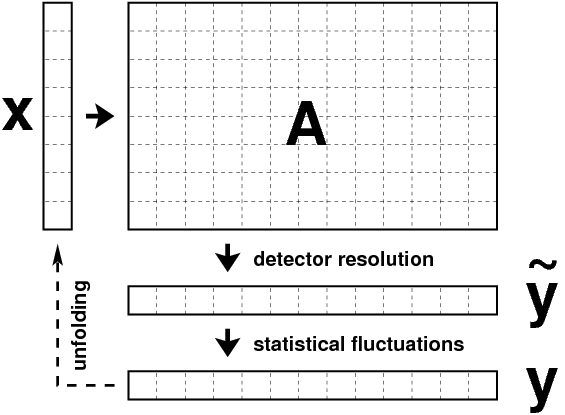
\includegraphics[width=0.4\textwidth]{06_DiffXsec/plots/d12-129f1.png}
  \caption{Schematic view of the problem of migration effects due to the finite precision of the detector and statistical 
  fluctuations. Plot taken from \cite{Schmitt:2012kp}.}
  \label{fig:scUnf}
\end{figure}

The most simple solution would be to take $y_{i}$ instead of $\tilde{y}_{i}$ in eq. \ref{eq:UnfoldProb} and invert
the $A_{ij}$ matrix to obtain $x_{j}$. But it turns out that the statistical fluctuations of $y_{i}$ are greatly 
amplified this way. To minify these fluctuations the \textit{regularisation} procedure is applied.

The process of restoring the true distribution $\tilde{x}_{j}$ from the known distribution $y_{i}$ which was influenced
by the detector effects and statistical fluctuations is called \textit{unfolding}. The TUnfold \cite{Schmitt:2012kp} algorithm was used for the
unfolding in this work.

\subsection{TUnfold Minimization}

The TUnfold algorithm is using the least square minimization method and the Tikhonov regularization \cite{Tikhonov:1963}. One of the crucial 
constrains for a better performance of the method is that the number of degrees of freedom for the minimization ($n - m$) has to be positive,
or $n > m$. This means that the true unfolded distribution $\tilde{x}_j$ will have coarser binning than the measured one, $y_{i}$.

The unfolding algorithm of the TUnfold determines the stationary point or minimum of the Lagrangian:

\begin{align}
 \mathcal{L}(x, \lambda) & = \mathcal{L}_{1} + \mathcal{L}_{2} + \mathcal{L}_{3}, \;\;\;\;\;\;\;\;\;\; \textrm{where}\\
 \mathcal{L}_{1} & = (\mathbf{y} - \mathbf{A}\mathbf{x})^{T} \mathbf{V_{yy}}^{-1}(\mathbf{y} - \mathbf{A}\mathbf{x}),\\
 \mathcal{L}_{2} & = \tau^{2}(\mathbf{x} - f_{b}\mathbf{x_{0}})^{T} (\mathbf{L^{T}L}) (\mathbf{x} - f_{b}\mathbf{x_{0}}), \\
 \mathcal{L}_{3} & = \lambda(Y -\mathbf{e}^{T}\mathbf{x}) \;\;\;\;\;\;\;\;\;\;\;\;\;\;\;\; \textrm{with} \\
 Y & = \sum_{i} y_{i}, \\
 e_{j} & = \sum_{i} A_{ij}.
\end{align}

The bold symbols here correspond to the matrices and vectors.

The term $\mathcal{L}_{1}$ is expected for the minimization. Vectors $\mathbf{y}$, $\mathbf{x}$ and a matrix $\mathbf{A}$ were
described in the previous section. Representing the migrations from and into different bins of $\mathbf{y}$, the matrix $\mathbf{A}$
is often defined from the Monte Carlo\footnote{A matrix $\mathbf{A}$ is
determined from Monte Carlo using the information from the generator particle level and on the reconstructed signal. An extra row is added
to the matrix $\mathbf{A}$ containing the information about the count of Monte Carlo events which were generated in some bin of $\mathbf{x}$,
but were not reconstructed in any of the $\mathbf{y}$ bins.}.
The $\mathbf{V_{yy}}$ is a covariance matrix of $\mathbf{y}$. 

The term $\mathcal{L}_{2}$ is responsible for the regularization. It is reducing the effect of the statistical fluctuations of $\mathbf{y}$
during the search of the stationary point of the Lagrangian $\mathcal{L}$. The $\tau^{2}$ is the regularization strength. Matrix $\mathbf{L}$
represents regularization conditions, having $n$ columns and $n_{R}$ rows which corresponds to $n_{R}$ conditions. $f_{b}$ is a normalization 
factor. In a very simple case $f_{b} = 0$, $\mathbf{L}$ is a unity matrix and $\mathcal{L}_{2} = \tau^{2} \parallel x \parallel^{2}$, which
suppresses the large deviations of $\mathbf{x}$ from zero. In case $f_{b} = 1$, the deviations of $\mathbf{x}$ from $\mathbf{x_{0}}$ are
suppressed. It is very important to choose the optimal regularization strength, as a very weak strength would not damp the fluctuation effects
from $\mathbf{y}$, whereas a very strong one will bias $\mathbf{x}$ towards $f_{b}\mathbf{x}_{0}$. The L-curve method \cite{Hansen00thel-curve} and the minimization
of correlation coefficients \cite{VBlobelT} are implemented in TUnfold for an optimal regularization strength choice. A multidimentional
regularization is possible in TUnfold.

The term $\mathcal{L}_{3}$ is an orthogonal area constrain with a Lagrangian parameter $\lambda$. If $\lambda$ is not set to zero,
which means the area constrain is used, the $\mathbf{x}$ is forced to match the total event count $Y$ correcting for the efficiencies $\mathbf{e}$.
This is used to limit the normalization biases if the data $\mathbf{y}$ follow Poisson's statistics \cite{Cowan98}.

The stationary point of the Lagrangian $\mathcal{L}(\mathbf{x}, \lambda)$ is defined by setting the first derivatives to zero. In case no 
area normalization is performed the Lagrangian $\mathcal{L}$ depends only on $\mathbf{x}$ and $\mathcal{L}_{3}$ term is zero.


%%%%%%%%%%%%%%%%%%%%%%%%%%%%%%%%%%%%%%%%%%%%
%%%%%%%%%%%%%%%%%%%%%%%%%%%%%%%%%%%%%%%%%%%%
%%%%%%%%%%%%%%%%%%%%%%%%%%%%%%%%%%%%%%%%%%%%
\section{Cross Section Definition}

After all the corrections are performed, the signal events grouped to different bins are used to define the normalized double differential cross sections
of the $t\bar{t}$ production process:

\begin{equation}\label{eq:ddxsecdef}
 (\frac{1}{\sigma} \frac{d\sigma}{dx\:dy})_{ij} = \frac{1}{\sigma} \frac{N^{signal}_{ij}}{\Delta x_{i}\Delta y_{j} \cdot BR \cdot L}
\end{equation}

Here $\sigma$ is a total cross section, $BR$ is a branching ratio of the $t\bar{t}$ dilepton decay channel and $L$ is the luminosity
collected by the CMS detector during the data taking 

% \subsection{Total Production Cross Section}
% \subsection{Double Differential Production Cross Section}